% easychair.tex,v 3.1 2011/12/30
%
% Select appropriate paper format in your document class as
% instructed by your conference organizers. Only withtimes
% and notimes can be used in proceedings created by EasyChair
%
% The available formats are 'letterpaper' and 'a4paper' with
% the former being the default if omitted as in the example
% below.
%
\documentclass[procedia]{easychair}
%\documentclass[debug]{easychair}
%\documentclass[verbose]{easychair}
%\documentclass[notimes]{easychair}
%\documentclass[withtimes]{easychair}
%\documentclass[a4paper]{easychair}
%\documentclass[letterpaper]{easychair}

% This provides the \BibTeX macro
\usepackage{doc}
\usepackage{makeidx}
\usepackage{multirow}
\usepackage{array}

% In order to save space or manage large tables or figures in a
% landcape-like text, you can use the rotating and pdflscape
% packages. Uncomment the desired from the below.
%
% \usepackage{rotating}
% \usepackage{pdflscape}

% If you plan on including some algorithm specification, we recommend
% the below package. Read more details on the custom options of the
% package documentation.
%
% \usepackage{algorithm2e}

% Some of our commands for this guide.
%
\newcommand{\easychair}{\textsf{gpnn}}
\newcommand{\miktex}{MiK{\TeX}}
\newcommand{\texniccenter}{{\TeX}nicCenter}
\newcommand{\makefile}{\texttt{Makefile}}
\newcommand{\latexeditor}{LEd}

\def\procediaConference{99th Conference on Topics of
  Superb Significance (COOL 2014)}

%\makeindex

%% Front Matter
%%
% Regular title as in the article class.
%
\title{A Computational Framework for Implementation of\\
       Neural Networks on Multi-Core Machine}

% \titlerunning{} has to be set to either the main title or its shorter
% version for the running heads. When processed by
% EasyChair, this command is mandatory: a document without \titlerunning
% will be rejected by EasyChair

\titlerunning{Computational Framework for Implementation of Neural Networks}

% Authors are joined by \and. Their affiliations are given by \inst, which indexes into the list
% defined using \institute
%
\author{
    Wenduo Wang\inst{1}%\thanks{Designed and implemented the class style}
\and
    Yi L. Murphey\inst{2}%\thanks{Masterminded EasyChair and created versions 3.0--3.4 of the class style}\\
}

% Institutes for affiliations are also joined by \and,
\institute{
  University of Michigan-Dearborn,
  Dearborn, Michigan, U.S.A\\
  \email{wenduow@umich.edu}
\and
   University of Michigan-Dearborn,
   Dearborn, Michigan, U.S.A\\
   \email{yilu@umich.edu}\\
}

%  \authorrunning{} has to be set for the shorter version of the authors' names;
% otherwise a warning will be rendered in the running heads. When processed by
% EasyChair, this command is mandatory: a document without \authorrunning
% will be rejected by EasyChair

\authorrunning{Wang and Murphey}

\begin{document}

\maketitle

\keywords{back-propagation, neural networks, parallel computing, multi-core machine, generic programming}

\begin{abstract}

This paper presents a computational framework, GPNN, for efficient implementation of Back-Propagation based neural learning algorithms running on multi-core machines.  GPNN has three components, parallelization of neural learning, abstraction of network components, and compile-time generalization.  The parallelization component decomposes the back-propagation learning algorithm into two stages, forward propagation and back-propagation.  During the forward propagation, training data are partitioned and distributed to K-threads, which run simultaneously multiple images of a neural network system on a multi-core machine. The back-propagation process, which runs on a single thread, collects the errors generated from the K-threads and uses it to update weights.  The abstraction component models input, bias, weight, and neuron as abstract nodes and abstract layers.  The compiler-time generalization component uses a generic programming technique to make neural network components instantiated at compiler time, which further reduces execution time. Together these computational components make GPNN an efficient framework for fast implementation of back-propagation based neural learning algorithms, and providing flexibility and reusability for modifying neural network topologies.  The GPNN was applied to four different neural learning algorithms, classic back-propagation (BP), quick propagation (QP), resilient propagation (RP) and Levenberg-Marquardt (LM) algorithm. Experiments are conducted to evaluate the effectiveness of GPNN, and results show that the neural learning algorithms implemented in GPNN are more efficient than their respective functions provided by Matlab.

\end{abstract}

%------------------------------------------------------------------------------

\section{Introduction}

Artificial neural networks are widely used in a wide range of research areas and shown being effective in solving many applications problems.  In recent years, many applications face the challenges of discovering and extracting knowledge from large and complex data.  However, as pointed by many researchers, our current machine learning methodologies and software tool are not sufficient to handle the volume, variability, and velocity of big data \cite{fan2013mining, labrinidis2012challenges}.  Computational efficient algorithms are key areas of research in dealing with big data.  The most noticeable software for processing big data is Apache Hadoop, a set of algorithms for distributed storage and distributed processing of very large data sets on computer clusters built from commodity hardware.  Hadoop was initially designed to focus on running massive MapReduce jobs to process a web crawl.  Recently Hadoop has been expanded to broad applications and ubiquitous usage, which has exposed some problems \cite{vavilapalli2013apache}.  There are also research activities focusing on fast implementation of neural learning algorithms such as FANN, OpenNN and tnnlib \cite{nissen2003implementation, lopezopennn}, which take advantages of generic programming, algorithm and topology diversity and parallel execution. This research focuses on exploring the potential of using creative software technology to maximize parallelism in implementation of back-propagation based neural learning algorithms, and create a programming environment that is efficient for research in neural learning from big data, which has strong need for flexibility in making changes in neural network topology and optimizing learning parameters used in back-propagation based neural networks through repeated experiments on big data.  Many important machine learning issues, for example, over-fitting, network size, memory space need for the end product, require the analysis of data generated from extensive experiments.

In this paper, we present a computational framework, GPNN, designed for efficient implementation of the back-propagation based neural networks. The GPNN consists of three computational components, parallelization of neural learning, abstraction of neural network components, and compile-time generalization.  The parallelization component decomposes the back-propagation learning algorithm into two stages, forward propagation and back-propagation.  During the forward propagation path, the training data are partitioned and distributed to $K$ threads, which all have identical images of the neural network.  The errors generated from the $K$ threads are combined and used for weight update through the back-propagation, which is running on a single thread.  This parallelization technique can improve training time considerably when training data are big.  The abstraction component provides techniques for representing neural network components input, bias, weight, neuron and target in abstract nodes and abstract layers.  The abstraction process provides an efficient architecture for implementing parallel computation in neural learning.  For example since weights are the only data needed in forward propagation and, under the abstraction process, they are represented in separate abstract layers, they can be easily copied or shared among multiple threads as network images.  The remaining parts of the network, i.e. input nodes, biases, neurons and target nodes, can stay local without being distributed over the multi-cores.  Therefore the abstraction process helps to reduce communication time and required memory size, which could be significant improvement over efficiency when processing big data using large systems.  The Compile-Time Generalization component uses generic programming technique to instantiate data types such as learning algorithms, transfer functions, error functions and network topologies at compiler time, which eliminates the run-time used in each loop to determine the running type of these objects.  Together these computational components in GPNN provides mechanisms for fast implementation of back-propagation based neural learning algorithms, flexibility and reusability for neural network research in studying neural network topologies and optimizing learning parameters.

We have implemented four neural learning algorithms in the GPNN framework, classic back-propagation (BP) \cite{boden2001guide}, quick propagation (QP) \cite(fahlman1988empirical), resilient propagation (RP) \cite{riedmiller1993direct} and Levenberg-Marquardt (LM) algorithm \cite{hagan1994training}.  Experiments are conducted to evaluate the effectiveness of GPNN by training these learning algorithm to solve a practical problem, predicting humidity based on features such as visibility, wind direction, dew point pressure, etc.  The run-time complexity of these algorithms are compared with their respective algorithms provided by Matlab.

This paper is organized as follows.  Section~\ref{section:implementation} introduces the three major components in GPNN, Section~\ref{section:performance} presents the experiment results and Section~\ref{section:conclusion} concludes the paper.

%------------------------------------------------------------------------------

\section{A Computational Framework for Implementing Back-Propagation based Neural Learning Algorithms}
\label{section:implementation}

The proposed computational framework, GPNN, is developed to optimize the implementation of back-propagation based neural networks using creative software techniques. Back-Propagation is the most popular neural learning algorithm for supervised learning in multi-layered feed-forward networks as well as in many recurrent neural networks.  Most of these neural networks have a unique forward path and back-propagation path.  The forward path is used to propagate the input from the input layer to the output layer, which can be represented as follows,

\begin{gather}
    net_j = \sum_i w_{ji} x_i \notag \\
    x_j = f_j(net_j) \notag
\end{gather}

where $x_i$ is the outputs from the neuron $i$ in previous layer, which is regarded as the inputs of neuron $j$, $w_{ji}$ is the weight from all previous neuron $i$ to neuron $j$, net is calculated as the weighted sum of all the inputs, and $x_j$ is the output after $net_j$ filtered by the transfer function $f_j$, which is also regarded as one of the input of next layer.

The backward path follows gradient descent calculated by the chain rule,

\begin{equation}
    \frac{ \partial E_j }{ \partial w_{ji} } = \frac{ \partial E_j }{ \partial x_j } \cdot \frac{ \partial x_j }{ \partial net_j } \cdot \frac{ \partial net_j }{ \partial w_{ji} } = \frac{ \partial E_j }{ \partial x_j } f'_j(net_j) x_i \text{.} \notag
\end{equation}

If the error function is chosen as the mean squared error in batch training mode, then it has the following expression,

\begin{equation}
    E_j = \frac{1}{2} \sum_d ( t_d - y_d ) ^ 2 \notag
\end{equation}

where $d$ contributes to each input training pattern, $|d|$ represents the total number of training pattern, $t_d$ is target, and $y_d$ is predicted output (same as the output $x_{j,d}$ of last layer).  The gradient can be calculated as follows,

\begin{align}
    \frac{ \partial E_j }{ \partial w_{ji} } & = \sum_d { \frac{ \partial { \frac{1}{2} ( t_d - y_d )^2 } }{ \partial y_d } f'_j ( net_{j,d} ) x_{i,d} } \notag \\
    & = - \sum_d { ( t_d - y_d ) f'_j ( net_{j,d} ) x_{i,d} } \text{.} \notag
\end{align}

For every hidden neuron, its gradient is affected by all of its successors.  To consistently express the gradient of output nodes and hidden nodes, let

\begin{equation}
    \delta_{ji,d} = \left \{
    \begin{array}{l l}
        t_d - y_d & \quad \text{for output neuron} \\
        \sum_k {w_{kj}\delta_{kj,d} } & \quad \text{for hidden neuron}
    \end{array} \right. \notag
\end{equation}

where $k$ contributes to next layer.

In software implementation, a classic neural network layer is normally modeled as a container, which holds a weight matrix, a bias node and multiple neurons.  Additionally, it specifies the propagation order of these components.  In a global view, layer can be connected with each other.
The following introduces the three major components in GPNN, parallelization of neural learning, abstraction of neural network components, and compile-time generalization.  We will also show, using an example, the flexibility of reconstruct a new neural network from an existing one in the GPNN framework.

\subsection{Parallelization of Neural Learning Algorithm}

According to Moore’s law, the density of circuits doubling at every new generation \cite{chu2007map}.  In the recent years, computer systems have increased the number of cores significantly to support parallel computing.  Particularly in big data applications, it is important to implement neural learning algorithms in high level of parallelization on multi-core CPUs with shared memory to achieve significant increases in CPU performance.  We propose an approach of multi-thread implementation of batch training BP \cite{schuessler2011parallel}, which is illustrated in Fig.~\ref{fig:parallelization}.  It is a $K$-thread parallel computing structure, in which a neural network is copies $K$ times, and the training data are partitioned and distributed to these $K$ threads.  Therefore the inputs are processed simultaneously along the feed-forward paths of these $K$ threads, and errors are collected at the end of each thread.  Then the errors at all $K$ threads are combined for weight update using gradient descent (back-propagation path), which is represented as follows,

\begin{equation}
    \frac{\partial E_j}{\partial w_{ji}} = \sum_k \frac{\partial E_j^{(k)}}{\partial w_{ji}^{(k)}} \text{.} \notag
\end{equation}

Weights are then all updated through the back-propagation process.  The updated neural network is made $K$ copies, and the same training process is repeated until user defined stop criteria are satisfied.

\begin{figure}[tb]
    \begin{centering}
        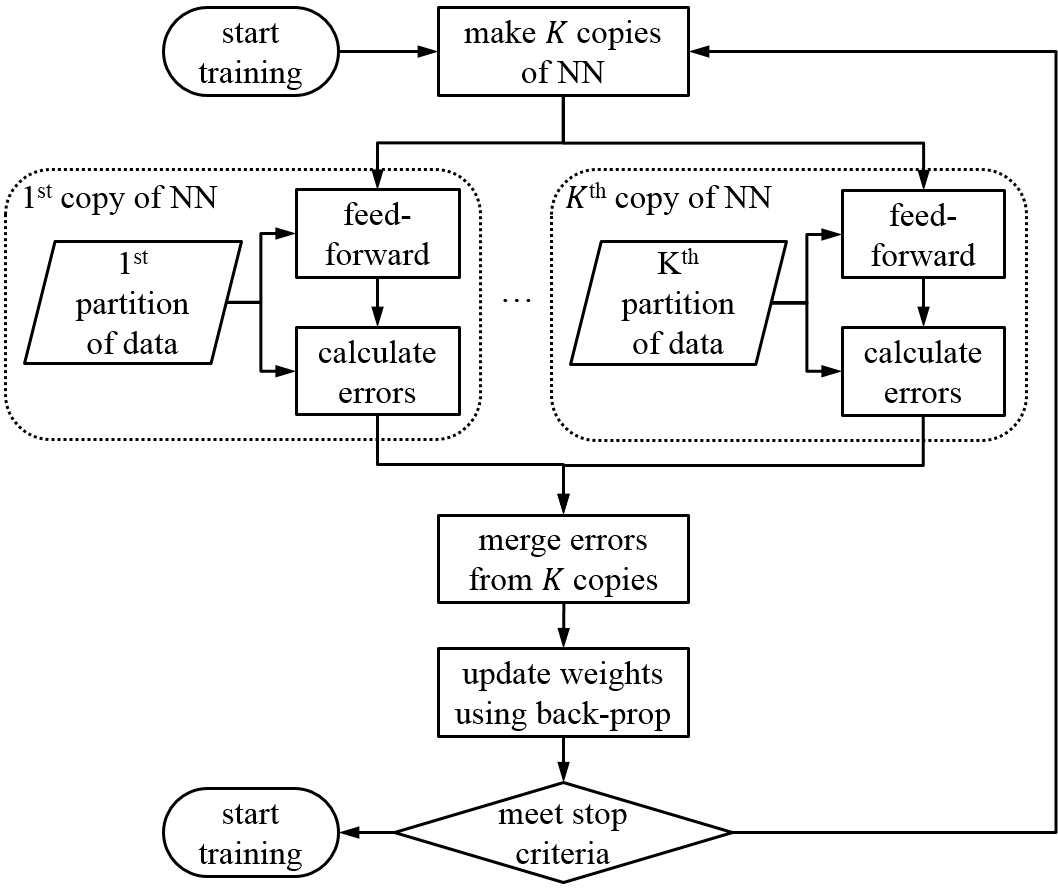
\includegraphics[scale=0.5]{../pic/parallelization.png}
        \caption{Illustration of multi-thread implementation of neural learning process.}
    \label{fig:parallelization}
	\end{centering}
\end{figure}

\subsection{Abstraction of Neural Network Components}

Abstraction is a very critical and powerful concept in object-oriented programming.  It treats objects with similar functions as the same module.  Based on this concept, weights between neurons can be considered as similar to neurons, since a neuron has one input axon and one output axon, and a weight connecting two neurons can also be considered to have an input, which is the output axon of the preceding neuron, and the weight can be considered as its output axon, which is connected to the input axon of following neuron.  The transfer function of a weight is defined as follows,

\begin{align}
    & \text{feed-forward:} & x_{ji} = f_{ji}(x_i) = w_{ji}x_i \notag \\
    & \text{back-propagation:} & \delta_j = w_{ji}\delta_{ji} \text{.} \notag
\end{align}

For the same reason, an input node to a neural network can also be treated as similar to a neuron, which has the equal number of output axons to the first hidden layer but no input axon.  Similarly, bias of a neuron layer can also be handled in this way.  There is no need for back-propagation from any of these input nodes.

\begin{align}
	& \text{feed-forward for input:} & x_i = f_0(p) = p \notag \\
	& \text{feed-forward for bias:} & x_b = f_b(1) = 1 \notag
\end{align}

where $p$ is the value of input feature, $x_i$ is the output of the input node, and the output of the bias node $x_b$ is always 1.

The output of a neuron is represented as a target node, which has one input axon connected to the output of a neural network, but no output axon, i.e., there is no feed-forward from a target node.

\begin{align}
    & \text{target node:} & \delta_j = t_j - y_j \notag
\end{align}

where $t_j$ is the target value of this output node, and $y_j$ is the network predicted value.  Target nodes are used in back-propagation process.

Based on the above discussion, input, bias, weight, neuron and target are all considered as nodes in an abstraction context.  Nodes of the same type are grouped into the same abstraction layer, and these abstracted layers are connected to each other as illustrated in Fig.~\ref{fig:nn_abstracted}, in which a one-layer of neurons in a neural network is represented by input abs-layer (abstraction layer), bias abs-layer, weight abs-layer, neuron abs-layer and target node abs-layer.  The connection among nodes and abstracted layer are considered equivalent in the context of programming.

\begin{figure}[tb]
    \begin{centering}
        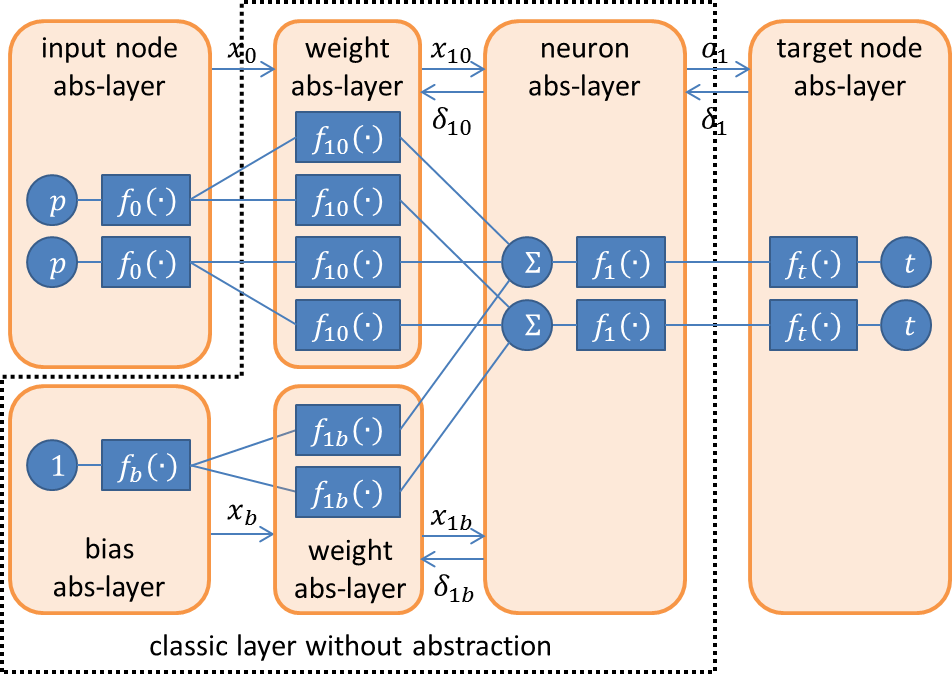
\includegraphics[scale=0.5]{../pic/nn_abstracted.png}
        \caption{One-layer of neural network topology represented by the abstraction layers (abs-layer).  The abstracted layers inside the box in dash-line is the neural network layer.}
        \label{fig:nn_abstracted}
	\end{centering}
\end{figure}

The abstraction process provides an efficient architecture for implementing parallel computation in neural learning, since only weights need to be copied or shared among multiple threads as network images.  In the abstraction process, weights are represented in separate abstract layers so they can be easily copies or shared without touching the other parts of the network, e.g., input nodes, biases, neurons and target nodes, which can stay local without being distributed over the multi-cores.  Therefore the abstraction approach can reduce communication cost, and reduce the need for memory.  This improvement could be significant in applications involving neural learning from big data.

Current input and output of a node are stored for each input pattern for weight update processing during the back-propagation.  Other values are prepared during feed-forward or back-propagation for intermediate calculation of critical variables, e.g., $f(net)$ and $f'(net)$ shown in Fig.~\ref{fig:microscopic}.

\begin{figure}[tb]
    \begin{centering}
        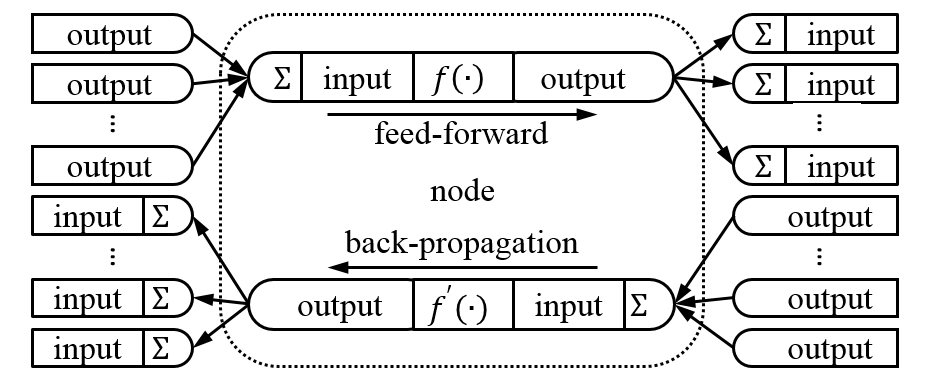
\includegraphics[scale=0.5]{../pic/microscopic.png}
        \caption{Communication between nodes during feed-forward and back-propagation.}
        \label{fig:microscopic}
	\end{centering}
\end{figure}

\subsection{Compile-Time Generalization}

Generic programming is a software approach that can be used to generalize replaceable functional nodes in neural networks.   In a generic programming architecture variables can be written in terms of types to-be-specified-later  \cite{wiki:generic_programming}, and then instantiated when needed.  In neural networks, transfer functions, network topologies, and weight update functions can be type-deduced so functional call can be determined during compile time  \cite{alexandrescu2001preface}.

We proposed to implement weights using compile-time generalization, since they used in different data types including forward, backward, update and copy processes.  User can specify an appropriate update strategy of weights during programming without modifying rest part of the code.  The compiler then generate a made-to-order target file related to the developer customized behavior data types.  In addition, since the software is tailored to specific behavior data types at compiling period, this implementation greatly reduces irrelevant code, thus, reduces the software size.   The compile-time generalization of weights eliminates the run-time otherwise needed in every loop to determine the running type of weight object through looking up its virtual table.

Fig.~\ref{fig:run_vs_compile} illustrates the differences between run-time and compile-time implementation of a neural learning process.  In the run-time generation implementation, weight type is deduced in every epoch, which means that the processors need to spend time on deciding weight type in each loop through looking up a virtual table.  As a consequence, the accumulative time consumed in all loops is conspicuous.  If the compile-time generalization implemented, data type deduction is calculated only once at the compiling process.  Moreover, if the neural network software is required to be run multiple times for different experimental purposes, run-time generalization time on type deduction can be more significant.  Contrarily, because there’s no need to compile the same neural network software again for repeated experiments, the compile-time generalization does not need extra time for data type deduction.  In summary, the time complexity for run-time generalization of weights is $O(mn)$, which can be saved if data type deduction for weights are carried out at the compiling process.

\begin{figure}[tb]
    \begin{centering}
        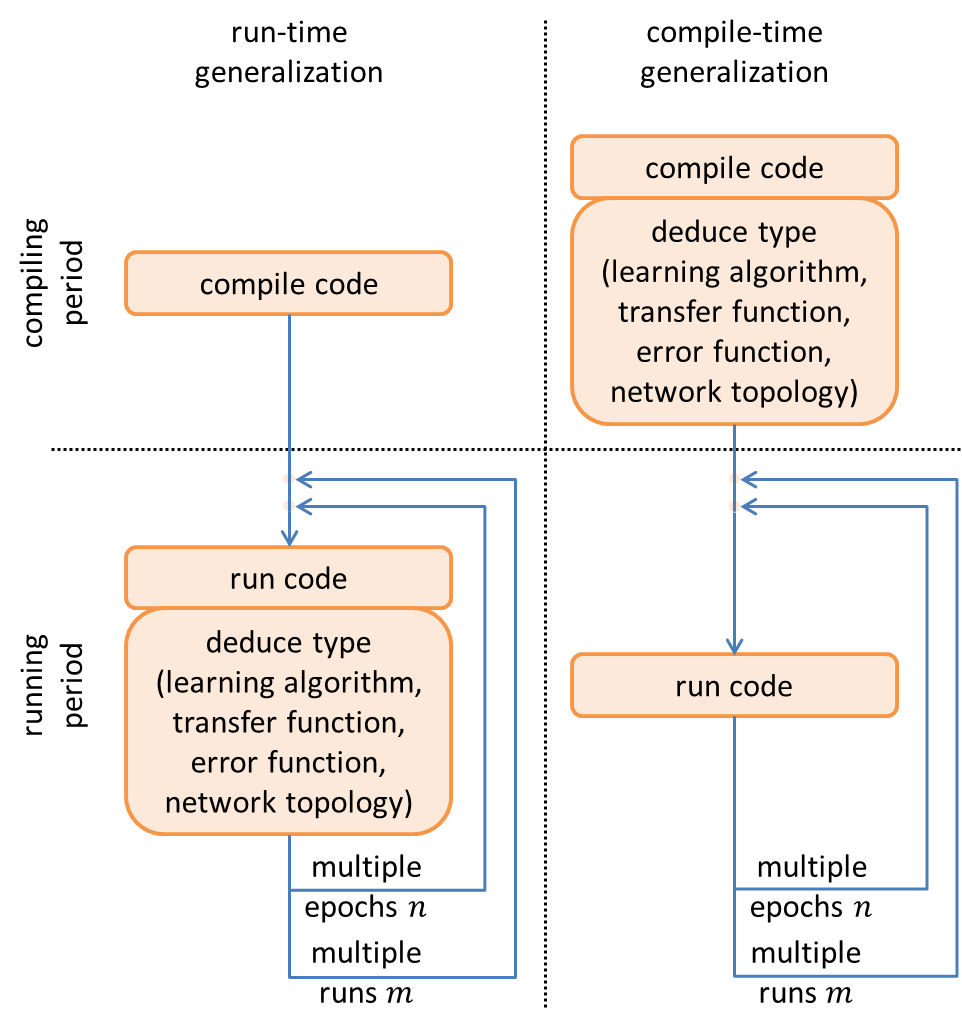
\includegraphics[scale=0.5]{../pic/run_vs_compile.png}
        \caption{Run-time generalization versus compile-time generalization during the processes of compiling code to running code for a neural learning algorithm.  Note $n$ is epoch number and $m$ is number of experiment repeated.}
        \label{fig:run_vs_compile}
	\end{centering}
\end{figure}

In terms of design pattern, the compile-time generalization approach is also known as policy based class design \cite{alexandrescu2001policy}.  In our implementation, a learning algorithm is defined as a type of update policy, a transfer function is defined as a type of transfer policy, a network topology is defined as a kind of topology policy, an error function is defined as a kind of error policy, and even the number of neurons, input, target and other training factors can be considered as individual policies as well.

\subsection{Flexibility and Reusability of GPNN Framework}

In addition to the fast implementation of neural learning algorithms, the proposed GPNN framework also provides flexibility and reusability for neural network research.  The abstraction and compile-time generalization processes in GPNN allow researchers to build new neural networks by simply connecting or pruning nodes, without the need of re-constructing the most part of an existing network architecture.  The following algorithm shows the steps to build a recurrent neural network, which has no bias, and uses LM algorithm and log-sigmoid transfer function, based on an existing biased one-layer neural network, which uses the BP algorithm and a linear transfer function.  Fig.~\ref{fig:reusability} illustrates the algorithm steps.

Building a recurrent neural network:

\begin{enumerate}
    \item Detach the bias abstracted layer and the weight abstracted layer in the given neural network.
    \item Attach a neuron abstracted layer using linear transfer function, and attach a weight abstracted layer using LM algorithm.
    \item Replace the algorithm type of the weight abstracted layer from BP to LM, and replace the transfer function type of the neuron abstracted layer from log-sigmoid to linear.
\end{enumerate}

\begin{figure}[h]
    \begin{centering}
        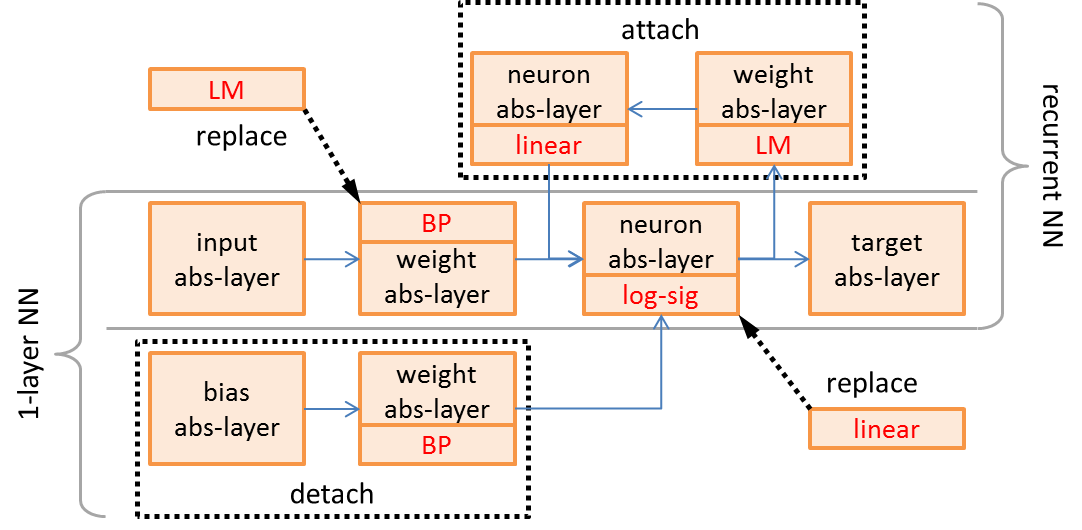
\includegraphics[scale=0.5]{../pic/reusability.png}
        \caption{Building a recurrent neural network by modifying a one-layer neural network.}
        \label{fig:reusability}
	\end{centering}
\end{figure}

%------------------------------------------------------------------------------

\section{Performance and Experiment Result}
\label{section:performance}

We applied the proposed computational framework, GPNN, to four back-propagation based neural learning algorithms, classic back-propagation (BP), quick propagation (QP), resilient propagation (RP) and Levenberg-Marquardt (LM) algorithm.

The QP takes the largest steps possible to reach local minima without overshooting.  The QP learning algorithm is based on the assumption that the error versus weight curve can be approximated by a parabola whose arms open upward \cite{fahlman1988empirical}, which means its second derivative is approximately linear with a positive slope k.  For a parabola curve, the minimum value is where its second derivative equals to 0.  QP is efficient for large training data.

The basic idea of RP is that every time the gradient changes its sign, it indicates that the last update was so big that the error function skipped a local minimum.  Thus, the weight update absolute value needs to be reduced by a factor $ \eta ^ - $, where $ 0 < \eta ^ - < 1 $.  Contrarily, if the gradient remains the same sign as previous update, a larger step of $\theta$ can be increased by factor  $ \eta ^ + $, where $ \eta ^ + > 1 $.  The detail of the RP algorithm can be found in \cite{riedmiller1993direct}.

The LM algorithm aims at solving non-linear least square problem.  It interpolates between the Gauss–Newton algorithm (GNA) and the method of gradient descent. The LM algorithm is more robust than the GNA \cite{hagan1994training}.

We implemented these four neural learning algorithms using the parallelization, abstraction and compiler-time generalization processes discussed in Section~\ref{section:implementation}.

In order to evaluate the performance of the proposed GPNN, we applied the following experiment data to the four neural learning algorithms implemented using GPNN. Experiment data are selected from hourly historical climate data of Ann Arbor, MI, USA and downloaded from \url{www.wunderground.com} website from year 2010 to 2013.  The data from year 2010 to 2012 were used as training data and year 2013 as testing data.  The total number of training samples is 26304, and total number testing samples is 8760.  The training samples are partitioned evenly and distributed to all the threads, the number of which is determined by the configuration of each experiment.  Ten input features listed in Table~\ref{table:climate} are input to each neural network system.  The neural network output is the predicted humidity value.  All input and output are normalized to zero mean ($ \mu = 0 $)and unit standard deviation ($ \sigma = 1 $).

\begin{table}[htp]
    \centering
    \caption{Features in Climate Dataset.}
    \begin{tabular}{ c l c c }
        \hline \hline
        Usage & Feature & Valid Range & Unit \\
        \hline
        \multirow{10}{*}{input}
            & month & 1 - 12 & - \\
            & hour & 0 - 23 & - \\
            & temperature & -50 - 150 & \(^\circ\)F \\
            & dew point & -50 - 150 & \(^\circ\)F \\
            & pressure & 28 - 31 & inHg \\
            & visibility & 0 - 10 & mile \\
            & wind direction & 0 - 359 & \(^\circ\) \\
            & wind speed & 0 - 50 & mph \\
            & gust speed & 0 - 100 & mph \\
            & precipitation & 0 - 1.5 & in \\
        \hline
        target & humidity & 0 - 100 & \% \\
        \hline \hline
    \end{tabular}
    \label{table:climate}
\end{table}

A computer with a 2.3GHz quad-core 8-thread CPU, 8G RAM, and a 64-bit operating system, was used to run all the experiments presented below.

\subsection{Evaluating Multi-Thread Efficiency}

Theoretically, multiple processors and cores can support almost any number of threads running simultaneously.  However, since the communication between threads is usually implemented by a pooling approach, it takes certain amount of time to synchronize all the image threads to main network thread.  It is clear that the most efficient number of threads should be equal to the number of cores, since running time of multi-threads on the same core will add up more than the running time of single thread even with thread scheduling applied.

The first experiment was conducted to evaluate different number of threads applied to different number of hidden nodes while BP was implemented using GPNN as a neural learning algorithm.  Fig.~\ref{fig:thread_efficiency} shows the training time for each of these neural network configurations running on different number of threads.  In these experiments, the stop criterion is to training until 2000 epoch was reached.  In order to get a robust measure, and every experiment was repeated 10 times and the average training time was presented.

\begin{figure}[tb]
    \centering
    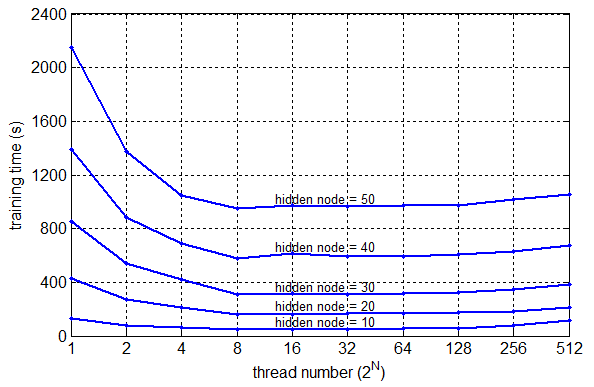
\includegraphics[scale=0.6]{../pic/efficiency.png}
    \caption{Training time of BP for different hidden node numbers versus different numbers of threads.}
    \label{fig:thread_efficiency}
\end{figure}

The result demonstrates that the fastest thread configuration is indeed 8 threads, which equals to the hardware concurrency of CPU in the computer.  It is about 3 times ($ \frac{132}{46} \approx 2.87 $) faster than training with single thread training a 10 hidden nodes network, but it is not able to obtain an ideal 8-time because of communication time cost as discussed earlier.  With the number of threads grows larger than 8, training time slightly goes up, which is due to the time cost for scheduling.

\subsection{Comparing GPNN Implementation with Conventional Implementation}

In this experiment, we compare the efficiency of the neural learning algorithms implemented using GPNN with their respective Matlab versions, except for the RP algorithm, which is not available in Matlab.  In this experiment, the stop criterion is also 2000 epochs, every experiment was repeated 10 times and the mean training time is presented in Table~\ref{table:algorithm_complexity}.

\begin{table}[htp]
    \centering
    \caption{Training Time at Different Thread Number.}
    \begin{tabular}{ l c c c c }
        \hline \hline
        Traing Time (s) & BP & QP & RP & LM \\
        \hline
        8-thread GPNN & 56.8 & 62.4 & 69.7 & 263.9 \\
        1-thread GPNN & 176.7 & 167.9 & 192.3 & 337.7 \\
        1-thread Matlab & 649.1 & - & 678.1 & 1264.0 \\
        \hline \hline
    \end{tabular}
    \label{table:algorithm_complexity}
\end{table}

It is no surprise that the 8-thread implementations of BP, QP and RP neural learning algorithms are much more computationally efficient than their respective 1-thread implementations.  It is noted that the LM algorithm is more time consuming than the other three neural learning algorithms.  This is because LM algorithm needs to calculate Hessian matrix inversion frequently during each iteration \cite{yu2011levenberg}.  Even the 8-thread implementation of LM algorithm does not reduce execution time much, which is due to the added time cost for communication among threads.  In the 1-thread implementation, the algorithms implemented in GPNN are much more efficient than their respective functions provided by Matlab, the speed up for the GPNN implemented BP is 3.6, the GPNN implemented QP is 3.5 times, and the GPNN LM is 3.7.

\subsection{Algorithm Efficiency based on Dynamic Stopping Criteria}

In many practices, neural network training could be terminated based on a number of dynamic criteria, for example, gradient approximates to 0, gradient stops decrease, and etc.  In this experiment, we train the GPNN implemented BP, QP, RP and LM learning algorithms using the following stopping criteria: when the mean error is less than $ 10 ^ {-9} $ or error has not changed for 6 epochs \cite{matlab:neural_networks}.  The configuration of the four neural networks are shown in Table~\ref{table:config_algorithm_efficiency}.  Each experiment is repeated 10 times and the average CPU times are presented in Table~\ref{table:algorithm_efficiency}.

\begin{table}[htp]
    \centering
    \caption{Neural Networks Configuration used in Algorithm Efficiency Analysis Experiments.}
    \begin{tabular}{ c c c c c }
        \hline \hline
        & BP & QP & RP & LM \\
        \hline
        thread number & 8 & 8 & 8 & 8 \\
        $\eta$ & 0.5 & 0.5 & - & - \\
        $\mu$ & - & 1.75 & - & - \\
        $\eta ^ -$ & - & - & 0.5 & - \\
        $\eta ^ +$ & - & - & 1.2 & - \\
        $\theta$ & - & - & 0.1 & - \\
        \hline \hline
    \end{tabular}
    \label{table:config_algorithm_efficiency}
\end{table}

\begin{table}[htp]
    \centering
    \caption{Training Time of Neural Learning Algorithms with Dynamic Stopping Criteria.}
    \begin{tabular}{ l c c c c }
        \hline \hline
        & BP & QP & RP & LM \\
        \hline
        training time (s) & 3.5 & 35.1 & 28.2 & 31.1 \\
        converge epoch & 43.2 & 976.4 & 866.7 & 97.2 \\
        training error (\%) & 3.80 & 1.86 & 0.73 & 3.15 \\
        testing error (\%) & 3.66 & 1.88 & 0.76 & 33.08 \\
        \hline \hline
    \end{tabular}
    \label{table:algorithm_efficiency}
\end{table}

The results show that LM algorithm converges in significantly less epochs than QP and RP.  However, it takes more time to run per epoch.  Although RP takes more epochs to converge, its training and testing errors are distinctly smaller than others.  The BP has the least training time and the least number of epochs, but its training and test error are the highest.  Based on these results we can deduce that if an application requires high accuracy, GPNN implemented RP algorithm is a good fit to find the local minima, and if big data are involved, LM is a good learning algorithm to use since it converges in the least number of epochs.

%------------------------------------------------------------------------------

\section{Conclusion}
\label{section:conclusion}

We have presented a computational framework, GPNN, for efficient implementation of back-propagation based neural learning algorithms for big data learning. In GPNN, the forward path of a neural network learning algorithm is distributed to K-threads, errors are then combined, and the weights updated by a back-propagation process running in a single thread.   The abstraction component in GPNN implements the abstractions of weights, neurons, transfer functions, input and output in terms of abstraction nodes, and organize the nodes into abstraction layers according to node types. The abstraction process provides an efficient computational environment for parallel computation during neural learning.  The GPNN also introduced a compile-time generalization technique to make as many neural network components being instantiated at compiler time as possible, which further reduces the execution time.

Experiments are conducted to evaluate the effectiveness of multi-thread implementation of GPNN implemented BP algorithm, and the comparison of computational time efficiency among the four neural learning algorithms, GP, QP, RP and LM, implemented using GPNN and the respective functions provided by Matlab library.  The experiment results show that the algorithms implemented in GPNN are more efficient than their respective functions provided by Matlab.  Specifically, the speed up for the GPNN implemented BP is 3.6, the GPNN implemented RP is 3.5 times, and the GPNN LM is 3.7.  When implemented in 8-thread parallelization with a fixed number of epochs as the training stopping criterion, the GPNN BP has the largest speed up, 3.1, over 1-thread GPNN BP, and LM algorithm has the least speed up, 1.3.  When the multiple stopping criteria of minimum error and error convergence are used, the results show that (1) although GPNN RP takes more epochs to converge, its training and testing errors are decidedly smaller than all others, (2) GPNN LM converges in less epochs than GPNN QP and GPNN RP, but it takes more time to run each epoch, and (3) the GPNN BP has the least training time, but its training and test error are the larger than all the other three.

Based on these results we conclude that GPNN RP algorithm is good to find minimum error, and GPNN LM is a good learning algorithm for big data applications.

In addition to efficient run-time, the proposed GPNN framework also provides flexibility and reusability for neural network research.  The abstraction and compile-time generalization processes in GPNN allow researchers to build new neural networks by simply connecting or pruning nodes without re-design the most part of an existing network architecture.

We have put the four neural learning algorithms implemented using the GPNN in a library available under LGPL license at \url{github.com/wenduow/BeefNet}.

%------------------------------------------------------------------------------

%\appendix

%% References with BibTeX database:

\bibliographystyle{plain}
\bibliography{gpnn}

\end{document}

% EOF

